\chapter{Proverb 20}
\begin{figure}
  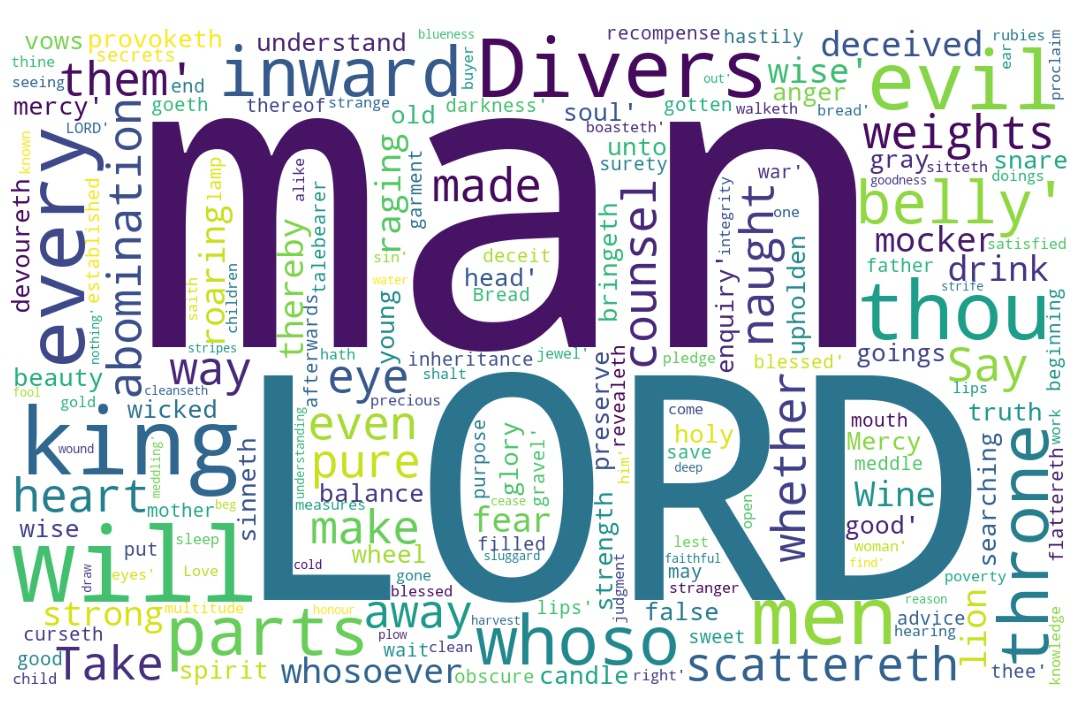
\includegraphics[width=\linewidth]{20OT-Proverbs/Proverb20-WordCloud.jpg}
  \caption{Proverb 20 Word Cloud}
  \label{fig:Proverb 20 word Cloud}
\end{figure}
\marginpar{\scriptsize \centering \fcolorbox{bone}{lime}{\textbf{PRINCIPLES TO OBSERVE}}\\ (Proverbs 20:1-30) \begin{compactenum}[I.][8]
    \item A \textbf{Fool and His Wine} \index[scripture]{Proverbs!Pro 20:01} (Pro 20:1)
    \item The \textbf{Fear of the King} \index[scripture]{Proverbs!Pro 20:02} (Pro 20:2) -- pay attention to those who can help you and those who can hurt you!
    \item \textbf{Fields Unplowed} \index[scripture]{Proverbs!Pro 20:04} (Pro 20:4) -- the bill for neglect comes with interest!
    \item The \textbf{Faithful Man Unseen} \index[scripture]{Proverbs!Pro 20:06} (Pro 20:6) -- when you find someone faithful (like a friend) hang on to that one
    \item \textbf{Finding Things out (with God's Help)} \index[scripture]{Proverbs!Pro 20:12} (Pro 20:12)
    \item The \textbf{Flatterer to Avoid} \index[scripture]{Proverbs!Pro 20:19} (Pro 20:19)
    \item The \textbf{False Balance Decried} \index[scripture]{Proverbs!Pro 20:23} (Pro 20:23) -- treat things with equity
\end{compactenum}}

\marginpar{\scriptsize \centering \fcolorbox{bone}{yellow}{\textbf{THE WORKS OF THE FOOL}}\\ (Proverbs 20:1-30) \begin{compactenum}[I.][8]
    \item Loses \textbf{Inhibitions} \index[scripture]{Proverbs!Pro 20:01} (Pro 20:1)
    \item Becomes an \textbf{Instigator} \index[scripture]{Proverbs!Pro 20:03} (Pro 20:3)
    \item Loves \textbf{Inactivity} \index[scripture]{Proverbs!Pro 20:04} (Pro 20:4)
    \item Possesses No \textbf{Integity} \index[scripture]{Proverbs!Pro 20:07} (Pro 20:7)
    \item Shows \textbf{Insincerity} \index[scripture]{Proverbs!Pro 20:19} (Pro 20:19)
    \item Has \textbf{Ingratitude} \index[scripture]{Proverbs!Pro 20:20} (Pro 20:20)
    \item Never Practices \textbf{Introspection} \index[scripture]{Proverbs!Pro 20:27} (Pro 20:27)
\end{compactenum}}

\footnote{\textcolor[cmyk]{0.99998,1,0,0}{\hyperlink{TOC}{Return to end of Table of Contents.}}}\footnote{\href{https://www.audioverse.org/english/audiobibles/books/ENGKJV/O/Prov/1}{\textcolor[cmyk]{0.99998,1,0,0}{Proverbs Audio}}}\textcolor[cmyk]{0.99998,1,0,0}{Wine \emph{is} a mocker, strong drink \emph{is} raging: and \fcolorbox{bone}{lime}{whosoever is deceived} thereby is not wise.}
[2] \textcolor[cmyk]{0.99998,1,0,0}{The \fcolorbox{bone}{lime}{fear of a king} \emph{is} as the roaring of a lion: \emph{whoso} provoketh him to anger sinneth \emph{against} his own soul.}
[3] \textcolor[cmyk]{0.99998,1,0,0}{\emph{It} \emph{is} an honour for a man to cease from strife: but every fool will be meddling.}
[4] \textcolor[cmyk]{0.99998,1,0,0}{The sluggard \fcolorbox{bone}{lime}{will not plow} by reason of the cold; \emph{therefore} shall he beg in harvest, and \emph{have} nothing.}
[5] \textcolor[cmyk]{0.99998,1,0,0}{Counsel in the heart of man \emph{is} \emph{like} deep water; but a man of \fcolorbox{bone}{MYGOLD}{understanding} will draw it out.}
[6] \textcolor[cmyk]{0.99998,1,0,0}{Most men will proclaim every one his own goodness: but a \fcolorbox{bone}{lime}{faithful man} who can find?}
[7] \textcolor[cmyk]{0.99998,1,0,0}{The just \emph{man} walketh in his integrity: his children \emph{are} blessed after him.}
[8] \textcolor[cmyk]{0.99998,1,0,0}{A king that sitteth in the throne of judgment scattereth away all evil with his eyes.}
[9] \textcolor[cmyk]{0.99998,1,0,0}{Who can say, I have made my heart clean, I am pure from my sin?}
[10] \textcolor[cmyk]{0.99998,1,0,0}{Divers weights, \emph{and} divers measures, both of them \emph{are} alike abomination to the LORD.}
[11] \textcolor[cmyk]{0.99998,1,0,0}{Even a child is known by his doings, whether his work \emph{be} pure, and whether \emph{it} \emph{be} right.}
[12] \textcolor[cmyk]{0.99998,1,0,0}{The \fcolorbox{bone}{lime}{hearing ear}, and the \fcolorbox{bone}{lime}{seeing eye}, the LORD hath made even both of them.}\footnote{\textbf{Proverb 25:2} - It is the glory of God to conceal a thing: but the honour of kings is to search out a matter.}
[13] \textcolor[cmyk]{0.99998,1,0,0}{Love not sleep, lest thou come to poverty; open thine eyes, \emph{and} thou shalt be satisfied with bread.}
[14] \textcolor[cmyk]{0.99998,1,0,0}{\emph{It} \emph{is} naught, \emph{it} \emph{is} naught, saith the buyer: but when he is gone his way, then he boasteth.}
[15] \textcolor[cmyk]{0.99998,1,0,0}{There is gold, and a multitude of rubies: but the lips of knowledge \emph{are} a precious jewel.}
[16] \textcolor[cmyk]{0.99998,1,0,0}{Take his garment that is surety \emph{for} a stranger: and take a pledge of him for a strange woman.}
[17] \textcolor[cmyk]{0.99998,1,0,0}{Bread of deceit \emph{is} sweet to a man; but afterwards his mouth shall be filled with gravel.}
[18] \textcolor[cmyk]{0.99998,1,0,0}{\emph{Every} purpose is established by counsel: and with good advice make war.}
[19] \textcolor[cmyk]{0.99998,1,0,0}{He that goeth about \emph{as} a talebearer revealeth secrets: therefore meddle not with him that \fcolorbox{bone}{lime}{flattereth} with his lips.}
[20] \textcolor[cmyk]{0.99998,1,0,0}{Whoso curseth his father or his mother, his lamp shall be put out in obscure darkness.}
[21] \textcolor[cmyk]{0.99998,1,0,0}{An inheritance \emph{may} \emph{be} gotten hastily at the beginning; but the end thereof shall not be blessed.}
[22] \textcolor[cmyk]{0.99998,1,0,0}{Say not thou, I will recompense evil; \emph{but} wait on the LORD, and he shall save thee.}
[23] \textcolor[cmyk]{0.99998,1,0,0}{Divers weights \emph{are} an abomination unto the LORD; and a \fcolorbox{bone}{lime}{false balance} \emph{is} not good.}
[24] \textcolor[cmyk]{0.99998,1,0,0}{Man's goings \emph{are} of the LORD; how can a man then understand his own way?}\footnote{\textbf{Jeremiah 17:9,10} - The heart is deceitful above all things, and desperately wicked: who can know it? [10] I the LORD search the heart, I try the reins, even to give every man according to his ways, and according to the fruit of his doings.}
[25] \textcolor[cmyk]{0.99998,1,0,0}{\emph{It} \emph{is} a snare to the man \emph{who} devoureth \emph{that} \emph{which} \emph{is} holy, and after vows to make enquiry.}
[26] \textcolor[cmyk]{0.99998,1,0,0}{A wise king scattereth the wicked, and bringeth the wheel over them.}
[27] \textcolor[cmyk]{0.99998,1,0,0}{The spirit of man \emph{is} the candle of the LORD, searching all the inward parts of the belly.}
[28] \textcolor[cmyk]{0.99998,1,0,0}{Mercy and truth preserve the king: and his throne is upholden by mercy.}
[29] \textcolor[cmyk]{0.99998,1,0,0}{The glory of young men \emph{is} their strength: and the beauty of old men \emph{is} the gray head.}
[30] \textcolor[cmyk]{0.99998,1,0,0}{The blueness of a wound cleanseth away evil: so \emph{do} stripes the inward parts of the belly.}



